% !TEX encoding = UTF-8
\documentclass[UTF8]{ctexart}

\usepackage[utf8]{inputenc}
\usepackage{graphicx}
\usepackage{geometry}
\geometry{a4paper}
\geometry{left=2.5cm,right=2.5cm,top=2.8cm,bottom=1.3cm}

\usepackage{booktabs}
\usepackage{array}
\usepackage{paralist}
\usepackage{verbatim}
\usepackage{subfig}
\usepackage{amsmath}
\usepackage{mathtools}
\usepackage{listings}
\usepackage[table]{xcolor}
\usepackage{lastpage}
\usepackage{url}

% Using hyperref for improved ref character
\usepackage[colorlinks,linkcolor=black,anchorcolor=black,
citecolor=black,CJKbookmarks=True]{hyperref}

% For picture drawing
\usepackage[all]{xy}

% For code inserting. Set features.
\lstset{
alsolanguage=matlab,
tabsize=4,
keepspaces=true,
numbers=left,
numberstyle=\tiny,
keywordstyle=\color{blue!70} \bfseries,
commentstyle=\color{red!50!green!50!blue!50},
frame=shadowbox,
breaklines,
showspaces=false,
showstringspaces=false,
showtabs=false,
rulesepcolor=\color{red!20!green!20!blue!20},
extendedchars=false,
escapeinside=``
}

% Set the font of page header
\usepackage{fancyhdr}
\pagestyle{fancy}
\lhead{传感器特性实验报告}
\chead{}
\rhead{Page \thepage/\pageref{LastPage}}
\cfoot{}
\rfoot{}
\lfoot{}

\usepackage{sectsty}

\usepackage[nottoc]{tocbibind}
\usepackage[titles,subfigure]{tocloft}
\renewcommand{\cftsecfont}{\rmfamily\mdseries\upshape}
\renewcommand{\cftsecpagefont}{\rmfamily\mdseries\upshape}

% Set number of ref to be relevent to section number
\renewcommand{\theequation}{\arabic{section}.\arabic{equation}}
\renewcommand{\thefigure}{\arabic{section}-\arabic{figure}}
\renewcommand{\thetable}{\arabic{section}-\arabic{table}}
\makeatletter
\@addtoreset{equation}{section}
\@addtoreset{figure}{section}
\@addtoreset{table}{section}
\makeatother

% Set the font of the reference
\bibliographystyle{unsrt}

% Define user\rq{}s color
\usepackage{colortbl}
\definecolor{lightgray}{gray}{.9}
\definecolor{thickgray}{gray}{.6}

\usepackage{multirow}

% 首行缩进
\usepackage{indentfirst}

% Set section numbering
\CTEXsetup[number={}]{part}
\renewcommand{\thepart}{}
\usepackage{titlesec}
\titleformat{\part}[block]{\color{blue}\huge\bfseries\filcenter}{}{1em}{}

%\usepackage{ulem}
%\usepackage{indentfirst}
%\setlength\textwidth{300.0pt}
%

% 重定义字体命令
\newcommand{\song}{\CJKfamily{song}}    % 宋体   (Windows自带simsun.ttf)
\newcommand{\fs}{\CJKfamily{fs}}        % 仿宋体 (华天字库htfs.ttf)
\newcommand{\kai}{\CJKfamily{kai}}      % 楷体   (华天字库htkai.ttf)
\newcommand{\hei}{\CJKfamily{hei}}      % 黑体   (Windows自带simhei.ttf)
\newcommand{\li}{\CJKfamily{li}}        % 隶书   (Windows自带simli.ttf)
\newcommand{\you}{\CJKfamily{you}}      % 幼圆体 (Windows自带simyou.ttf)
%%%  以上六种字体均为标准 GBK 字体, 包括 GBK 繁体字和一些不常用字, 推荐!!!

\newcommand{\xs}{\CJKfamily{xs}}
\newcommand{\shu}{\CJKfamily{shu}}      % 舒体   (方正字库fzstk.ttf)
%  \newcommand{\yourcommand}[参数个数]{内容}   [参数个数]这个是可选的。
%  例如  \newcommand{\you}{\CJKfamily{you}}  用\you 来代替 \CJKfamily{you} ,少输入很多字哦。
%字号设置
\newcommand{\chuhao}{\fontsize{42pt}{\baselineskip}\selectfont}
\newcommand{\xiaochuhao}{\fontsize{36pt}{\baselineskip}\selectfont}
\newcommand{\yihao}{\fontsize{28pt}{\baselineskip}\selectfont}
\newcommand{\xiaoyihao}{\fontsize{24pt}{\baselineskip}\selectfont}
\newcommand{\erhao}{\fontsize{21pt}{\baselineskip}\selectfont}
\newcommand{\xiaoerhao}{\fontsize{18pt}{\baselineskip}\selectfont}
\newcommand{\sanhao}{\fontsize{15.75pt}{\baselineskip}\selectfont}
\newcommand{\sihao}{\fontsize{14pt}{\baselineskip}\selectfont}
\newcommand{\xiaosihao}{\fontsize{12pt}{\baselineskip}\selectfont}
\newcommand{\wuhao}{\fontsize{10.5pt}{\baselineskip}\selectfont}
\newcommand{\xiaowuhao}{\fontsize{9pt}{\baselineskip}\selectfont}
\newcommand{\liuhao}{\fontsize{7.875pt}{\baselineskip}\selectfont}
\newcommand{\qihao}{\fontsize{5.25pt}{\baselineskip}\selectfont}
% \baselineskip | distance from bottom of one line of a paragraph to bottom of the next line.  基本行距
%  只有使用\selectfont命令之后,\fontzize{}{}的设置才能生效
%  可以用数字表示{11pt}:单倍行距

\begin{document}
%%%%%%%%%%%%%%%%%%%%%%%%%%%%封面与目录%%%%%%%%%%%%%%%%%%%%%%%%%%%%%%
\begin{titlepage}
\begin{center}
% Upper part of the page

\includegraphics[width=0.25\textwidth]{resource/logo.jpg}\\[1cm]
\textsc{\LARGE Department of Automation}\\[1.5cm]
\fs{\Large 模式识别基础第三次作业}\\[0.5cm]
% Title
\hrulefill
\\[0.8cm]{\centering \huge \hei 用身高体重数据进行性别分类的实验(三)}\\[0.4cm]
\hrulefill
\\[4cm]

% Author and supervisor
\begin{tabbing}       %tabbing  列表

 \hspace*{5cm} \= \hspace{2.6cm} \= \kill
 % \=     in tabbing environment, sets a tab stop
 % \kill  in a\tabbing environment, deletes previous line so tabs can be set without outputting text.
 % \>     in tabbing environment is a forward tab.

\>{\fs\sihao\textbf {班\hspace{1cm}级 \ \ :}}\>  {\centering\fs\sihao\textbf{~~~~~~~~~自~~3~2}} \\
\\
\>{\fs\sihao\textbf {姓\hspace{1cm}名 \ \ :}}\>  {\centering\fs\sihao\textbf{~~~~~~~~陈~昊~楠}}\\
\\
\>{\fs\sihao\textbf {学\hspace{1cm}号 \ \ :}}\>  {\centering\fs\sihao\textbf{~~~~~~2013011449}}\\
\\
\>{\fs\sihao\textbf {授课教师 \ \ :}}\>  {\centering\fs\sihao\textbf{~~~~~~~~张~学~工}} \\

\end{tabbing}
\vfill
{\large \today}
\end{center}
\end{titlepage}

\tableofcontents
\clearpage

%%%%%%%%%%%%%%%%%%%%%%%%%%正文部分%%%%%%%%%%%%%%%%%%%%%%%%%%%%%%%%%%

\section{实验内容}
	\begin{enumerate}
	\item 用 {\ttfamily dataset3} 作为训练数据,采用适当的特征选择方法选择$1\sim3$个特征采用不同的特征,采用适当的分类方法进行分类器设计,考查训练错误率;将设计出的分类器应用到{\ttfamily dataset4} 上,考查测试错误率。
	\item (选做)用某种K-L变换对{\ttfamily dataset3} 的10维特征进行变换,提取2 维新特征进行分类器设计(方法自选),对{\ttfamily dataset4} 也提取同样的2 维特征,测试分类器,与本次和前两次实验的结果进行适当的比较分析。
	\end{enumerate}

\section{特征选择方法概述}
一般的特征选择问题的解决思路是,构造一个准则函数,对一组特征打分,并搜索使得准则最优的特征组合。这种方式搜索空间很大,实际问题中可以采用如下几个思路:
\begin{enumerate}
\item 对每个特征,单独计算一个特征与目标分类的函数$f(X_i, y)$,该函数的值被称为p值。根据这个值对特征进行排序,并选择最优的几个特征。
\item 从一个特征集合中尝试删去部分特征,构造树状结构,并使用分支定界法进行搜索。
\item 与分类器集成在一起,而不是采用单独的可分性准则。例如{\ttfamily SVM-RFE}方法。
\end{enumerate}
实验中对这些思路都进行了尝试。另外,还实验了{\ttfamily PCA}降维的方法。

\section{实验结果}
	\subsection{特征数目对分类结果的影响}
	实验中使用对单个特征的F-检验,选取不同数目的特征,运用多种分类器检验分类效果。训练集准确率如表\ref{tab:nfeaturetrain},测试集准确率如表\ref{tab:nfeaturetest}。

	\begin{table}[htbp]
	\centering
	\begin{tabular}{cccccc}
	\toprule
	Features &   Bayes &     LDA &    LSVM & RBF SVM &     MLP \\
	\midrule
	9 &  90.88\% &  90.88\% &  90.99\% &  99.90\% &  91.51\% \\
	8 &  90.78\% &  90.78\% &  90.88\% &  98.43\% &  91.82\% \\
	7 &  90.67\% &  91.09\% &  90.88\% &  96.23\% &  90.88\% \\
	6 &  90.57\% &  90.99\% &  91.09\% &  93.29\% &  91.09\% \\
	5 &  90.57\% &  90.88\% &  91.19\% &  92.03\% &  91.51\% \\
	4 &  91.09\% &  90.46\% &  91.19\% &  91.93\% &  91.09\% \\
	3 &  90.99\% &  90.67\% &  90.99\% &  91.93\% &  90.88\% \\
	2 &  86.16\% &  87.95\% &  86.16\% &  87.95\% &  87.95\% \\
	1 &  87.84\% &  87.84\% &  87.84\% &  87.95\% &  87.95\% \\
	\bottomrule
	\end{tabular}
	\caption{不同特征数目下训练集准确率}
	\label{tab:nfeaturetrain}
	\end{table}

	\begin{table}[htbp]
	\centering
	\begin{tabular}{cccccc}
	\toprule
	Features &   Bayes &     LDA &    LSVM & RBF SVM &     MLP \\
	\midrule
	9 &  86.59\% &  90.55\% &  89.02\% &  85.06\% &  88.72\% \\
	8 &  86.28\% &  90.55\% &  89.02\% &  86.28\% &  89.02\% \\
	7 &  86.28\% &  90.55\% &  89.02\% &  87.80\% &  89.33\% \\
	6 &  86.28\% &  90.55\% &  89.02\% &  88.41\% &  90.85\% \\
	5 &  86.28\% &  90.85\% &  88.72\% &  87.50\% &  89.94\% \\
	4 &  86.89\% &  90.24\% &  88.72\% &  87.50\% &  88.72\% \\
	3 &  87.80\% &  89.63\% &  88.41\% &  88.41\% &  89.63\% \\
	2 &  81.71\% &  89.02\% &  81.71\% &  89.94\% &  89.94\% \\
	1 &  89.02\% &  89.02\% &  89.02\% &  89.02\% &  89.02\% \\
	\bottomrule
	\end{tabular}
	\caption{不同特征数目下测试集准确率}
	\label{tab:nfeaturetest}
	\end{table}

	由表可看出,在训练集上,准确率随特征数目的变化和分类器有一定关系,但基本上在使用$3\sim 7$个特征的情况下分类效果比较好。值得注意的是,{\ttfamily RBF SVM} 分类器的训练集准确率随特征数目的减少而单调减小。在测试集上情况比较复杂,特征变化也基本不是单调的。综合考虑准确率和计算量,选取3个特征比较好。以下的实验中都选取3个特征进行实验。

	\subsection{基于p值的特征选择}
	实验中使用了三种p值的选取方法。$\chi^2$检验方法、$F$检验方法和互信息量方法。在训练集上准确率如表\ref{tab:pvaluetrain},测试集上准确率如表\ref{tab:pvaluetest}。

	\begin{table}[htbp]
	\centering
	\begin{tabular}{cccccc}
	\toprule
	Method &   Bayes &     LDA &    LSVM & RBF SVM &     MLP \\
	\midrule
	$\chi^2$ test &  90.57\% &  91.19\% &  91.09\% &  91.93\% &  91.09\% \\
	$F$ test &  90.99\% &  90.67\% &  91.30\% &  91.93\% &  90.88\% \\
	MI &  90.25\% &  90.67\% &  91.30\% &  91.93\% &  90.88\% \\
	\bottomrule
	\end{tabular}
	\caption{不同p值函数下训练集准确率}
	\label{tab:pvaluetrain}
	\end{table}

	\begin{table}[htbp]
	\centering
	\begin{tabular}{cccccc}
	\toprule
	Method &   Bayes &     LDA &    LSVM & RBF SVM &     MLP \\
	\midrule
	$\chi^2$ test &  86.59\% &  90.55\% &  88.11\% &  87.80\% &  90.85\% \\
	$F$ test &  87.80\% &  89.63\% &  88.72\% &  88.41\% &  89.63\% \\
	MI &  87.80\% &  89.94\% &  88.72\% &  88.41\% &  88.72\% \\
	\bottomrule
	\end{tabular}
	\caption{不同p值函数下测试集准确率}
	\label{tab:pvaluetest}
	\end{table}

	由上表可看出,这三种p值方法的选择效果差不多。

	\subsection{基于模型的特征选择}
	实验中采用不同的分类方法尝试分类,并采用交叉检验的方法对模型进行检验。使用的分类方法有{\ttfamily Logistic} 回归,线性{\ttfamily SVM},采用L1参数正则化的线性{\ttfamily SVM}和决策树分类器。在训练集上准确率如表\ref{tab:modeltrain},测试集上准确率如表\ref{tab:modeltest}。其中前4行采用的方法是{\ttfamily RFE}方法递归剔除特征,且最终固定选择3个特征,后4行依据交叉检验结果选择最优个数的特征。

	\begin{table}[htbp]
	\centering
	\begin{tabular}{cccccc}
	\toprule
	Model &   Bayes &     LDA &    LSVM &  RBF SVM &     MLP \\
	\midrule
	Logistic &  84.17\% &  91.30\% &  91.30\% &   91.82\% &  90.88\% \\
	LSVM, L2 regulize &  90.99\% &  90.67\% &  91.30\% &   91.93\% &  90.88\% \\
	LSVM, L1 regulize &  82.70\% &  89.10\% &  91.30\% &   93.19\% &  91.51\% \\
	Tree &  90.57\% &  91.19\% &  91.30\% &   91.93\% &  90.88\% \\
	\midrule
	Logistic &  89.73\% &  91.19\% &  91.09\% &   92.14\% &  91.19\% \\
	LSVM, L2 regulize &  90.99\% &  90.25\% &  91.09\% &   91.82\% &  91.30\% \\
	LSVM, L1 regulize &  90.36\% &  90.88\% &  91.19\% &  100.00\% &  92.24\% \\
	Tree &  91.09\% &  90.46\% &  91.09\% &   91.93\% &  91.09\% \\
	\bottomrule
	\end{tabular}
	\caption{不同分类模型下训练集准确率}
	\label{tab:modeltrain}
	\end{table}

	\begin{table}[htbp]
	\centering
	\begin{tabular}{cccccc}
	\toprule
	Model &   Bayes &     LDA &    LSVM & RBF SVM &     MLP \\
	\midrule
	Logistic &  78.66\% &  90.24\% &  87.50\% &  89.33\% &  89.94\% \\
	LSVM, L2 regulize &  87.80\% &  89.63\% &  88.72\% &  88.41\% &  89.63\% \\
	LSVM, L1 regulize &  77.44\% &  86.59\% &  88.72\% &  88.41\% &  89.33\% \\
	Tree &  87.80\% &  90.55\% &  88.72\% &  88.41\% &  89.63\% \\
	\midrule
	Logistic &  87.20\% &  90.55\% &  88.11\% &  87.50\% &  88.11\% \\
	LSVM, L2 regulize &  88.72\% &  90.55\% &  88.72\% &  87.50\% &  88.11\% \\
	LSVM, L1 regulize &  86.59\% &  89.63\% &  87.80\% &  85.06\% &  87.50\% \\
	Tree &  86.89\% &  90.24\% &  88.72\% &  87.50\% &  88.72\% \\
	\bottomrule
	\end{tabular}
	\caption{不同分类模型下测试集准确率}
	\label{tab:modeltest}
	\end{table}

	与基于统计量的方法相比,基于模型并做交叉检验的方法计算量更大,且在实验使用的数据集上没有明显差别。由于该数据集一共只有10个特征,选择余地比较小,各种方法得到的结果都差不多。

	\subsection{特征重要性}
	不同方法获得的特征重要性如图\ref{fig:feature_importance}。

	\begin{figure}
	\centering
	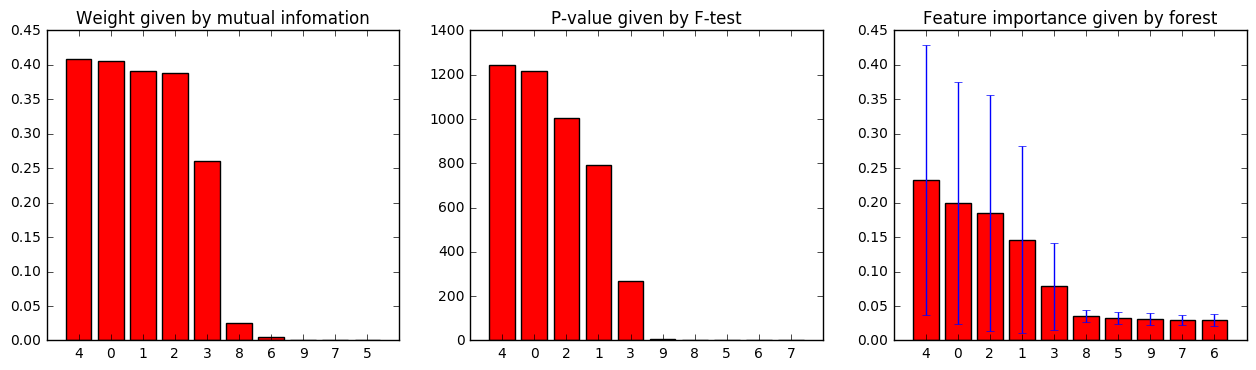
\includegraphics[width=16cm]{resource/feature_importance.png}
	\caption{以任意两个特征为横纵坐标的训练数据分布图}
	\label{fig:feature_importance}
	\end{figure}

	\subsection{PCA降维}
	{\ttfamily PCA}是一种特殊的$K-L$变换,使用单位矩阵作为变换核。实验中使用{\ttfamily PCA}将特征降至2维,训练集、测试集准确率如表\ref{tab:pca},在主成分上的类别分布如图\ref{fig:pca_decomposition}。由表可见,降维后准确率没有明显下降。
	\begin{table}[htbp]
	\centering
	\begin{tabular}{cccccc}
	\toprule
	{} &   Bayes &     LDA &    LSVM & RBF SVM &     MLP \\
	\midrule
	train &  89.94\% &  89.83\% &  89.94\% &  90.88\% &  90.04\% \\
	test  &  87.50\% &  87.50\% &  87.80\% &  89.33\% &  89.94\% \\
	\bottomrule
	\end{tabular}
	\caption{PCA降维训练集与测试集准确率}
	\label{tab:pca}
	\end{table}

	\begin{figure}
	\centering
	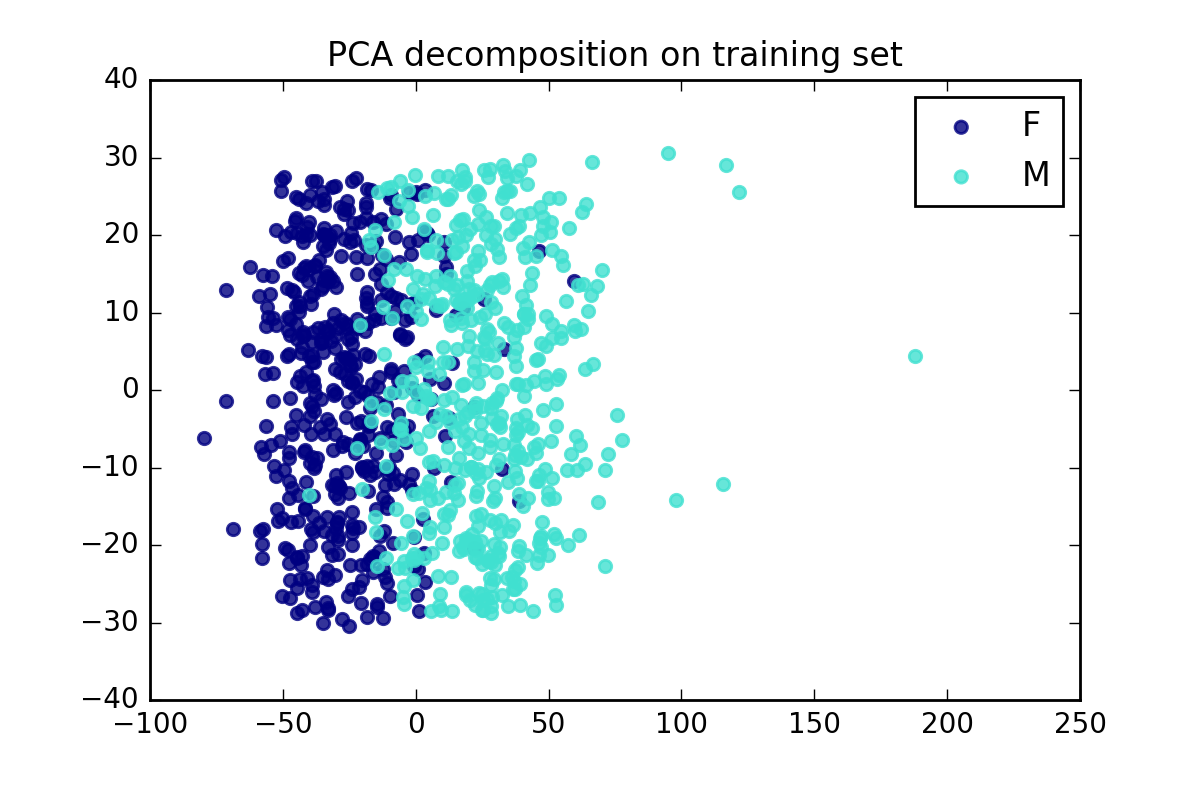
\includegraphics[width=11cm]{resource/pca_decomposition.png}
	\caption{PCA降维特征空间}
	\label{fig:pca_decomposition}
	\end{figure}

\section{分析与体会}
\begin{enumerate}
\item 本次实验中大量使用了库函数。比起之前的几次作业只能实现一部分实验的情况,这次作业很方便地进行了大量的对比实验。这说明实际应用中应该多使用库函数,提高效率。
\item 实验中的特征数目较少,难以比较各种特征选择方法。另外,最终的准确率和分类器也有很大关系。在模式识别系统中,特征选择和分类器需要有效配合才能达到较好的效果。
\end{enumerate}

\section{程序代码及说明}
程序使用{\ttfamily Python} 编写,使用{\ttfamily scikit learn} 的分类和特征选择库。源代码参见 \url{https://github.com/chaonan99/university_homework/blob/pattern_recognition/h3/src/h3.ipynb}

\end{document}
